\subsection{Grundlagen und Theorie}

Mit Hilfe einer sogenannten H-Brücke lassen sich die Wicklungen eines
Motors auf eine einfache Art und Weise ansteuern.\\

\begin{figure}[H]
    \centering
    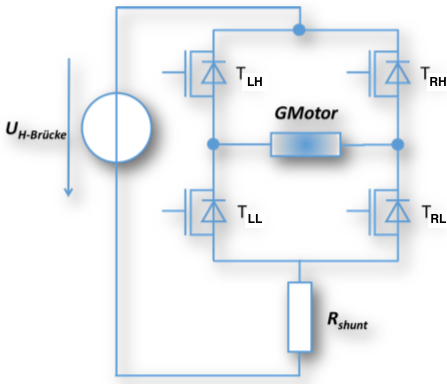
\includegraphics[width=1\textwidth]{schaltung_h_bruecke.png}
    \caption{Schaltung H-Brücke}
    \label{fig:Schaltung H-Bridge}
\end{figure}

Um den Strom positiv, also von links nach rechts, fließen zu lassen,
müssen die MOSFETS $T_{LH}$ und $T_{RL}$ angesteuert werden.\\

Wenn diese beiden besagten Transistoren ausgeschaltet werden, treibt die Energie im
Magnetfeld der Spule den Strom weiter. Dadurch fließt der Motorstrom $I_M$
durch die parasitären Bodydioden der Transistoren $T_{LL}$ und $T_{RH}$.\\

Dieser Strom kann indirekt durch die Spannung die über den Messwiderstand
$R_{Shunt}$ gemessen werden.\\

Soll der Motor in die entgegengesetzte Richtung betrieben werden, müssen
die MOSFETS $T_{RH}$ und $T_{LL}$ angesteuert werden.\\

Dadurch gibt es insgesamt 4 Zustände. Links-Rechts Transistoren an oder
ausgeschaltet und Rechts-Links Transistoren an oder ausgeschaltet.\\

Um die H-Brücke zu betreiben wird eine Steuerung benötigt. Die Steuerung
benötigt als Eingänge den Sollstrom $I_{soll}$ und den momentanen Strom
$I_{ist}$. Als Ausgänge 




% 2.2 
% Durch die Drehung des Motors wird eine Spannung Induziert. Dadurch fließt ein Strom durch die 
% sogenannten Parasit"ardioden T_RH und T_LL. 

% 2.3
% Der Strom l"asst sich "uber R_shunt messen, welcher passenderweise mit 1 OHM gew"ahlt ist. So ist
% die Spannung, die an R_shunt abf"allt gleich des Stromes.

% 2.4
% Es gibt vier verschiedene Zust"ande. Wenn der Motor im Uhrzeigersinn betrieben werden soll, k"onnen
% die entsprechenden Transistoren geschaltet sein oder nicht geschaltet sein. Soll der Motor gegen
% den Uhrzeigersinn betrieben werden, kann das andere Transistorenpaar geschaltet sein oder nicht.

% 2.5
% Eing"ange: I_IST, I_Soll, U_H-Br"ucke
% Ausg"ange: U_Motor

% 2.6
% 1. Fall: AN
%     U_H = U_T_LH + U_Motor + U_T_RL + U_R_shunt

%     U_H = R_LH * I_m + (R_shunt * I_m)  

% 2. Fall: Aus
%     0 = U_H + U_D + U_Motor + U_D + U_shunt